\subsubsection{Activity Diagram - Chức năng thêm dữ liệu từ file Excel}
\begin{figure}[H]
        \centering
        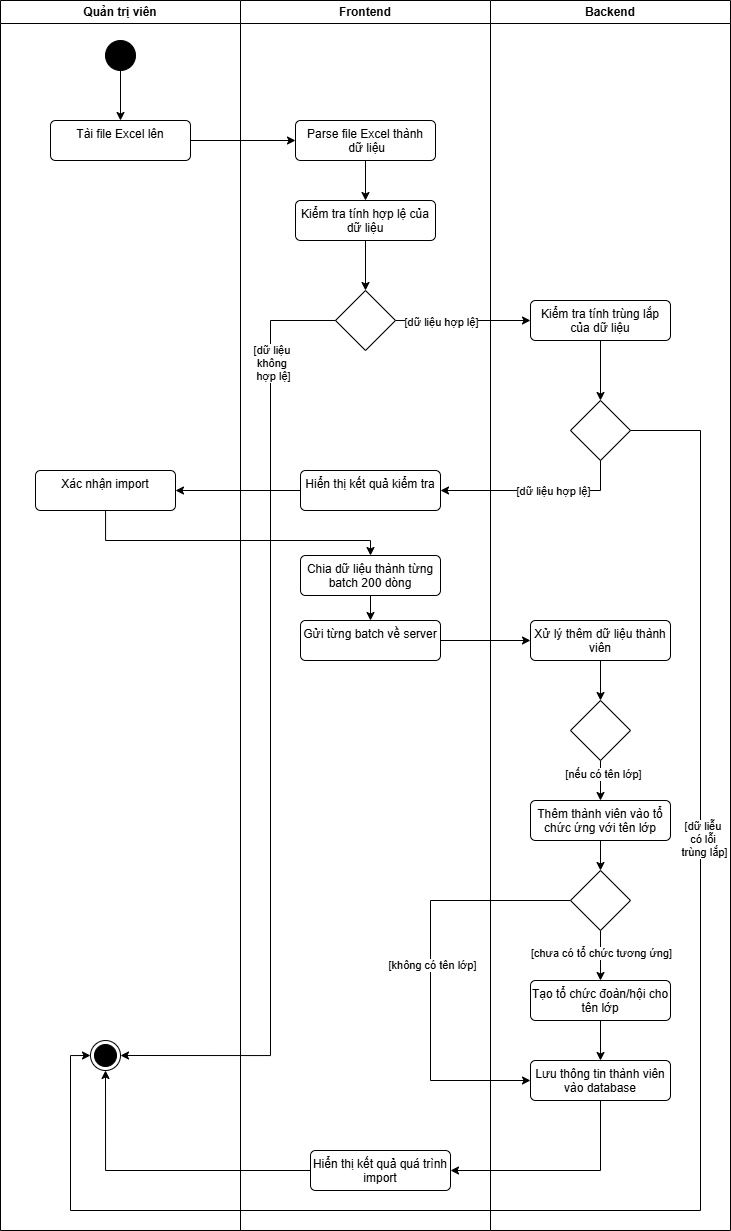
\includegraphics[width=0.75\linewidth]{Images/activity-diagram/import_from_file.png}
        \vspace{0.3em}
        \captionsetup{skip=8pt}
        \caption{Activity Diagram - Thêm nhiều thành viên từ file Excel}
        \label{fig:activity-uc04}
\end{figure}

Chức năng thêm dữ liệu từ file Excel trong module User được xây dựng nhằm hỗ trợ việc nhập nhanh số lượng lớn dữ liệu sinh viên vào hệ thống, đặc biệt trong giai đoạn đầu mỗi năm học khi cần cập nhật thông tin cho nhiều khóa và lớp khác nhau. Do đặc thù dữ liệu của các module quản lý như User, Department và Class là không đồng nhất, mỗi module có quy trình import riêng phù hợp với cấu trúc dữ liệu tương ứng. Trong phạm vi chức năng này, nhóm tập trung mô tả quy trình import dữ liệu tại module User do đây là module có tần suất sử dụng cao và đóng vai trò trung tâm trong việc quản lý thành viên.

Khi quản trị viên tải lên file Excel, hệ thống tiến hành đọc, kiểm tra dữ liệu đầu vào và xử lý từng dòng tương ứng với một người dùng. Với mỗi bản ghi, hệ thống tự động xác định và tạo cấu trúc tổ chức phù hợp dựa trên thông tin lớp học và khoa đào tạo. Cụ thể, hệ thống kiểm tra sự tồn tại của các tổ chức cấp khoa (level 2) và cấp lớp (level 3); trong trường hợp chưa tồn tại, hệ thống sẽ tự động khởi tạo mới. Tổ chức cấp cao nhất (level 1) là Đoàn trường hoặc Hội Sinh viên luôn được sử dụng làm tổ chức gốc để đảm bảo tính thống nhất trong mô hình tổ chức.

Sau khi hoàn tất việc xác định và tạo tổ chức, người dùng được tự động gán vào tất cả các tổ chức liên quan, bao gồm cấp trường (level 1), cấp khoa (level 2) và cấp lớp (level 3), với vai trò mặc định là \textit{MEMBER}. Hệ thống áp dụng logic xác định khoa đào tạo dựa trên mã lớp: nếu tên lớp bắt đầu bằng các tiền tố \textit{CC}, \textit{CN}, \textit{CT} hoặc \textit{TT}, sinh viên sẽ được gán vào \textit{Văn phòng Đào tạo Quốc tế}; các trường hợp còn lại sẽ xác định khoa dựa trên mã \textit{trainingDepartment} trong dữ liệu đầu vào.

\textbf{Ví dụ minh họa:}
\begin{itemize}[leftmargin=2em]
    \item \textbf{Mã lớp \textit{MT22KH02}}: Hệ thống xác định khoa đào tạo là \textit{Khoa Khoa học và Kỹ thuật Máy tính}, từ đó tạo (hoặc lấy) tổ chức cấp 2 là \textit{Liên chi đoàn/ Liên chi hội Khoa Khoa học và Kỹ thuật Máy tính} và tổ chức cấp 3 là \textit{Chi đoàn/ Chi hội lớp MT22KH02}.
    
    \item \textbf{Mã lớp \textit{CC23KTO1}}: Do mã lớp bắt đầu bằng tiền tố \textit{CC}, hệ thống xác định khoa đào tạo là \textit{Văn phòng Đào tạo Quốc tế}, đồng thời tạo (hoặc lấy) tổ chức cấp 2 là \textit{Liên chi đoàn/ Liên chi hội Văn phòng Đào tạo Quốc tế} và tổ chức cấp 3 là \textit{Chi đoàn/ Chi hội lớp CC23KTO1}.
\end{itemize}